\documentclass{article}

\usepackage[utf8]{inputenc}
\usepackage[T1]{fontenc}
\usepackage[french]{babel}
\usepackage{tabularx}
\usepackage{graphicx}
\usepackage{fullpage}

\title{Module AOC
\\
--
\\
Métronome}
\author{Thibaud Destouches \& Marceau Lacroix}
\date{2012 - 2013}

\begin{document}

\begin{titlepage}
\maketitle
\tableofcontents
\end{titlepage}

\newpage
\section{Introduction}
Le projet de métronome consiste en la conception et l'implémentation d'une architecture pour l'application métronome. Le métronome est décrit comme "un appareil qui emet un signal sonore ou lumineux à une fréquence donnée". La première version de cette application est d'une part un moteur de métronome et d'autre part une Interface Homme-Machine (IHM) pour ce moteur. La deuxième version vide au développement d'un adaptateur pour le métronome afin de "brancher" celui-ci sur une interface materielle (simulée). La troisième version (que nous ne devons pas réaliser) est l'utilisation de l'interface matérielle sur le moteur logiciel défini dans la V1. La réalisation de ce projet nous a confronté à la mise en oeuvre de plusieurs patrons de conception de manière simultannée et coopérative (Command et adapter implémenté par nous et observer implémenté par swing pour les listener). 

\section{Architecture}
\subsection{Version 1}
Cette première version du métronome utilise une IHM java "standard" (swing). Il s'agit d'une interface active, c'est à dire que l'interface notifie le controler lorsque l'un des composant impliquant un changement pour le métronome est utilisé. (changement de tempo, de taille de mesure, marche/arret)


\subsection{Version 2}
Pour cette deuxième version, l'interface devient complètement passive. Elle ne peut donc plus notifier le controleur des changements, c'est à lui de venir vérifier qu'un changement à eu lieu.





\section{Choix techniques et Ajouts}
\subsection{Choix techniques}
TODO


\subsection{Ajouts/Améliorations}
\begin{itemize}
\item \textbf{Visualisateur de mesure}: Ayant tous les deux déjà utilisé un métronome, nous avons décidé d'ajouter un "compteur" pour les mesures; ce compteur permet à l'utilisateur de savoir où en est la mesure en cours grâce à une barre de progression des temps dans la mesure. Au niveau de l'architecture, cet ajout à été très simple, nous avons juste ajouté deux appels de méthode dans l'IHM "de base": un dans le toc temps (pour remplir la barre d'un cran) et un dans toc mesure (pour vider la barre)
\item \textbf{Desactivations des boutons}: Afin d'améliorer l'experience utilisateur, nous avons choisi de désactiver les boutons lorsque l'action associé n'est pas disponible (par exemple, le bouton d'incrément de mesure est désactivé lorsque la mesure fait 7 temps).
\item \textbf{Compteur de mesure}: toujours dans le but d'améliorer l'experience utilisateur, nous avons choisi d'afficher le nombre de temps que comporte la mesure. L'ajout de cette fonctionnalité est quasiment "gratuite" en terme de temps de développement et apporte une information importante pour l'utilisateur.
\end{itemize}

\section{Tests}


\section{Conclusion}
L'utilisation d'une interface passive pour la V2 nous à obligé à rennoncer aux fonctionnalités "bonus" que nous avions dévoloppé pour la première version (notament l'afficheur de mesure) mais le sujet était clair à ce sujet.
Contrairement au projet de Master 1 (mini éditeur de texte) le métronome nous aura permis de réaliser que java est rapidement limité lorsque l'on essaye de jouer du son en "temps réel". On notera aussi que, contrairement à la plupart des autres projets que nous avons à réaliser cette année, les spécifications du métronomes étaient très claires.

\newpage
\section*{Annexes}
\begin{figure}[h]
   \caption{Diagramme de classes de la V1}
   
\includegraphics[scale=0.75]{class_diagram_v1}
\end{figure}
\begin{figure}[h]
   \caption{Diagramme de séquence de la V1: démarage du métronome}
   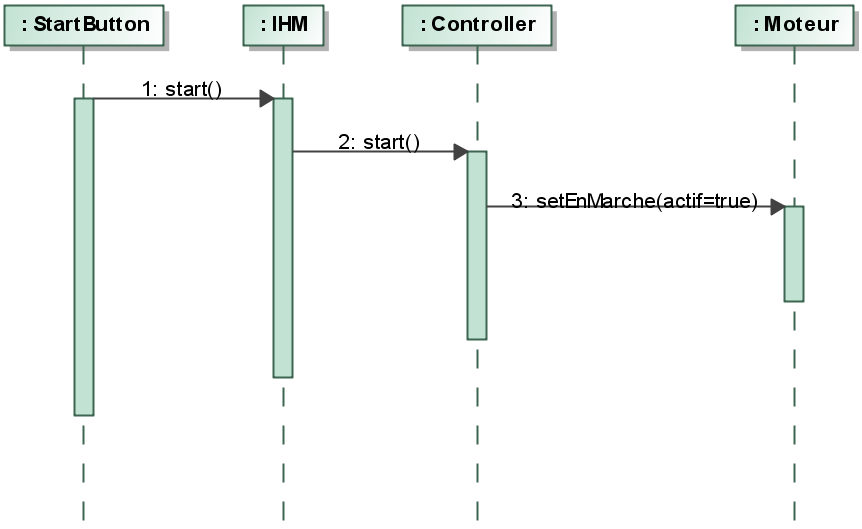
\includegraphics[scale=0.55]{seq_diagram_v1}
\end{figure}

\begin{figure}[h]
   \caption{Diagramme de classes de la V2}
   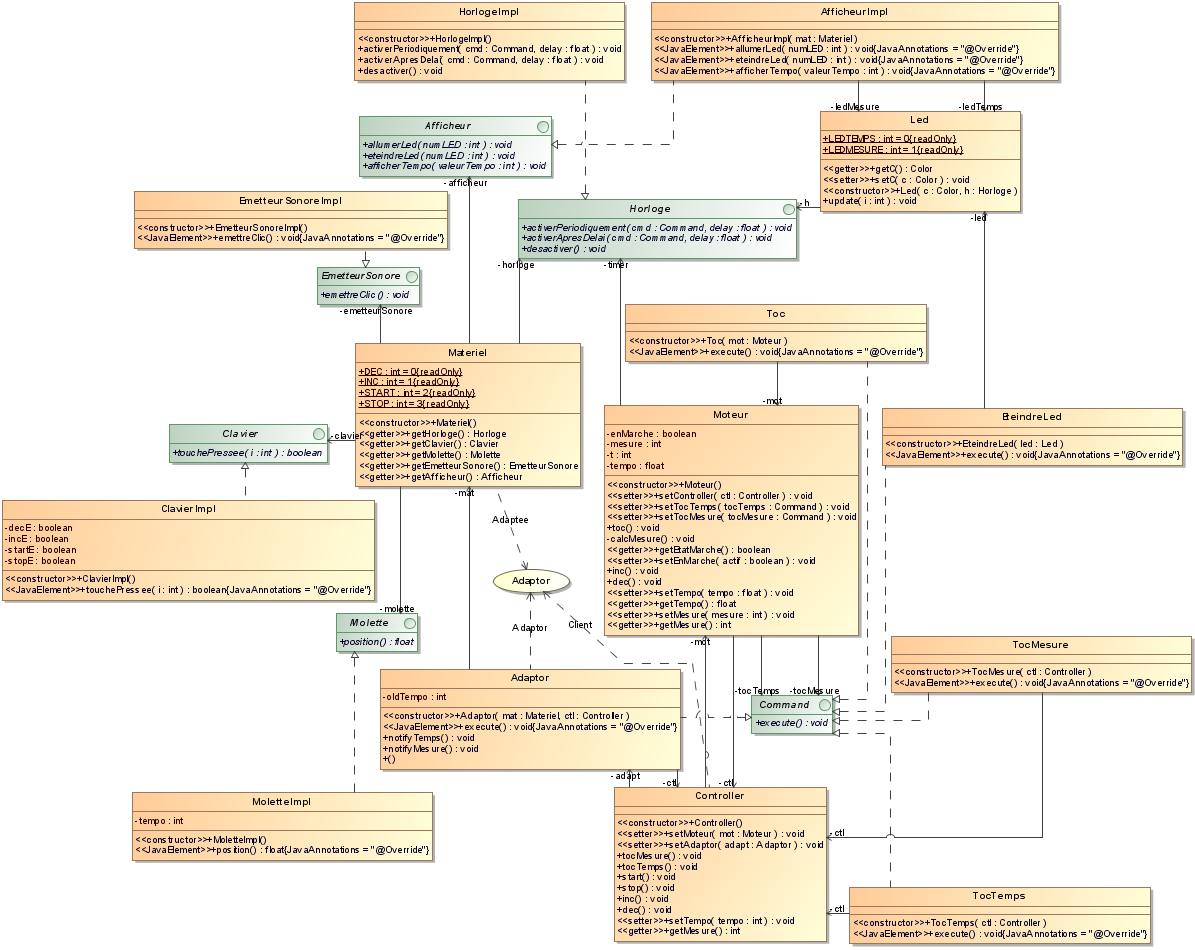
\includegraphics[scale=0.75]{class_diagram_v2}
\end{figure}
\begin{figure}[h]
   \caption{Diagramme de séquence de la V2: diminution de la mesure}
   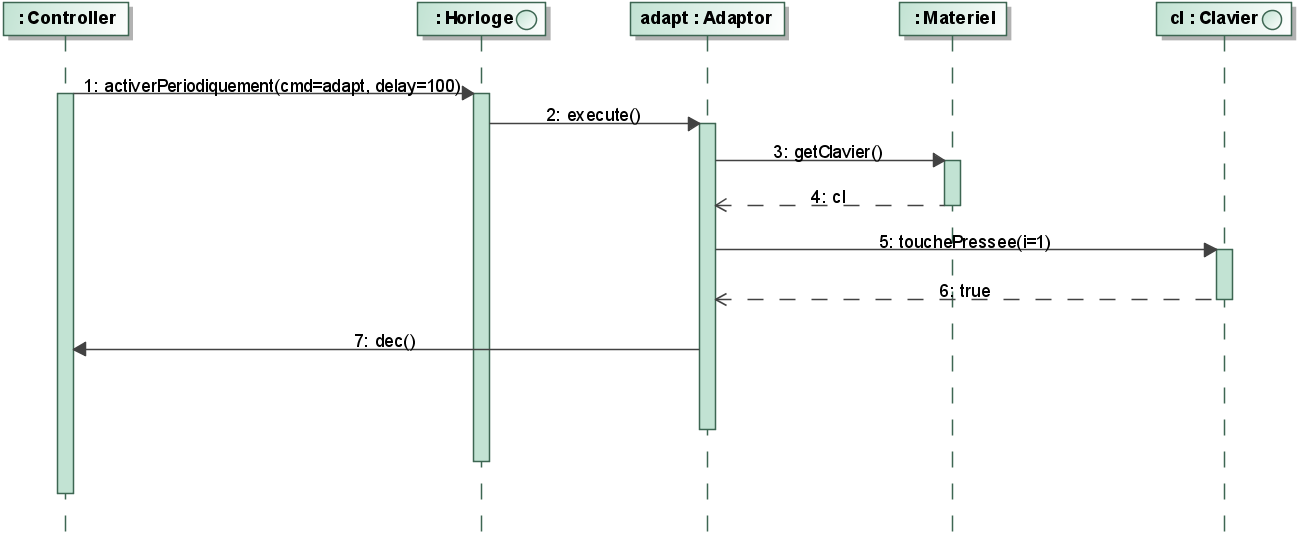
\includegraphics[scale=0.5]{seq_diagram_v2}
\end{figure}
\begin{figure}[h]
   \caption{Diagramme de séquence de la V2: "toc temps"}
   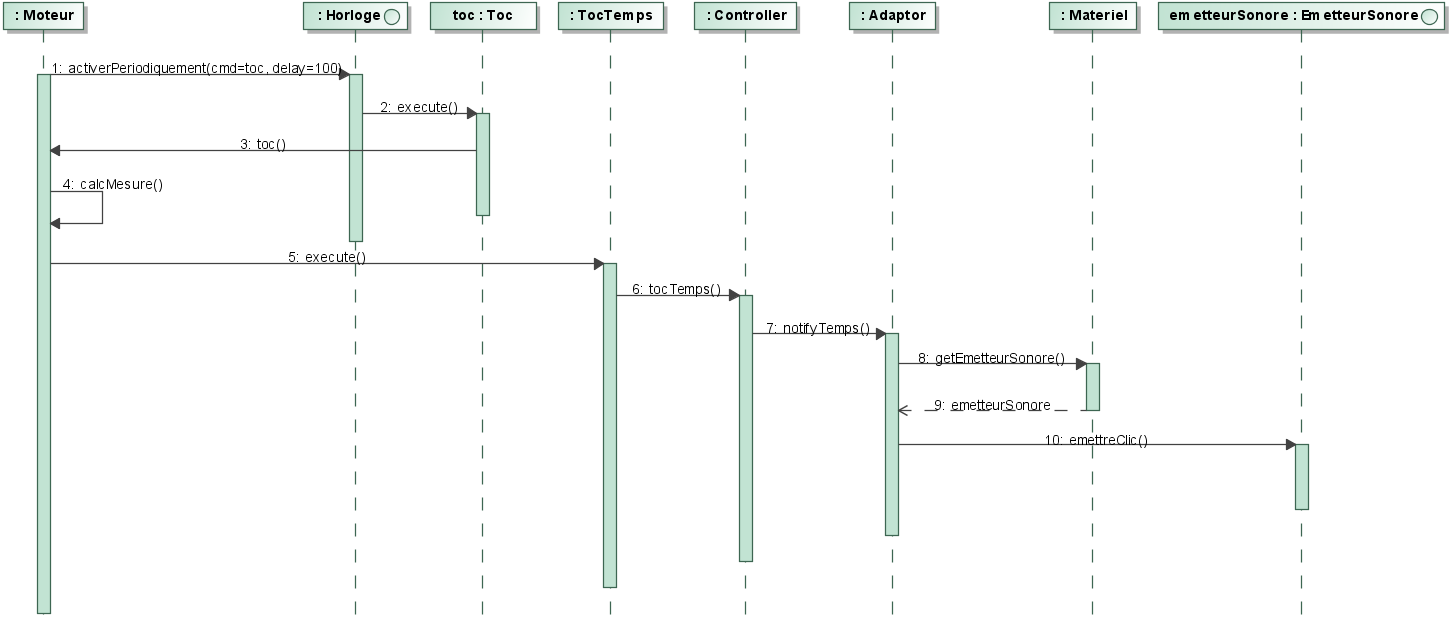
\includegraphics[scale=0.48]{seq_diagram_v2_2}
\end{figure}


\end{document}
